\documentclass[a4paper,10pt]{article}
%\usepackage[utf8x]{inputenc}
%\usepackage{czech}
\usepackage[utf8]{inputenc}
\usepackage[czech]{babel}
\usepackage{graphicx}

\title{Zpráva k seminární úloze z předmětu\\ Inteligentní robotika \\ {\small Zpráva č. 2 - Detekce komára v obraze a pohyb v jeho směru}}
\author{Filip Jareš, Lenka Mudrová}
\date{3.4.2011}

\begin{document}

\maketitle
\newpage

%Udelat titulni stranu!

\section{Popis úlohy}

Řešená úloha je inspirována článkem Backyard star wars \cite{clanek}. Pohyblivá kamera sleduje simulovaného komára, který je představován černým čtvercem na bílém pozadí monitoru. Pohyb kamery je možné řídit natočením okolo svislé osy (změnou azimutu) a natočením okolo vodorovné osy (změnou elevace). Cílem úlohy je řídit kameru tak, aby sledovala pohyb komára a zdokumentovala jeho „sestřel“ sérií snímků, ve kterých je komár ve středu obrazu z kamery – uprostřed „záměrného kříže“.

\section{Rozbor problému}

\section{Změny specifikace}

\section{Řešení problému}

Rámec programu je tvořen zpětnovazební regulační smyčkou pro řízení polohy kamery. Vstupem regulátoru je nejnovější získaný obrázek z kamery a jeho výstupem je nová poloha kamery. Schematicky je to znázorněno na obrázku \ref{fig:rid_system}.
Před samotným výpočtem nové polohy kamery je vyhodnocen nově získaný obraz. Postup jeho zpracování je znázorněn na obrázku \ref{fig:kamera}.
Nejprve je určena poloha komára v obraze (funkce \textit{findMosquitoInImage}) v pixelových souřadnicích. Na základě odchylky této polohy od středu obrázku potom funkce \textit{mosquitoPxPositionToAzimuthAndElevation} počítá odhad úhlů, o které je komár vychýlen od optické osy kamery.

\begin{figure}[!h]
    \centering
     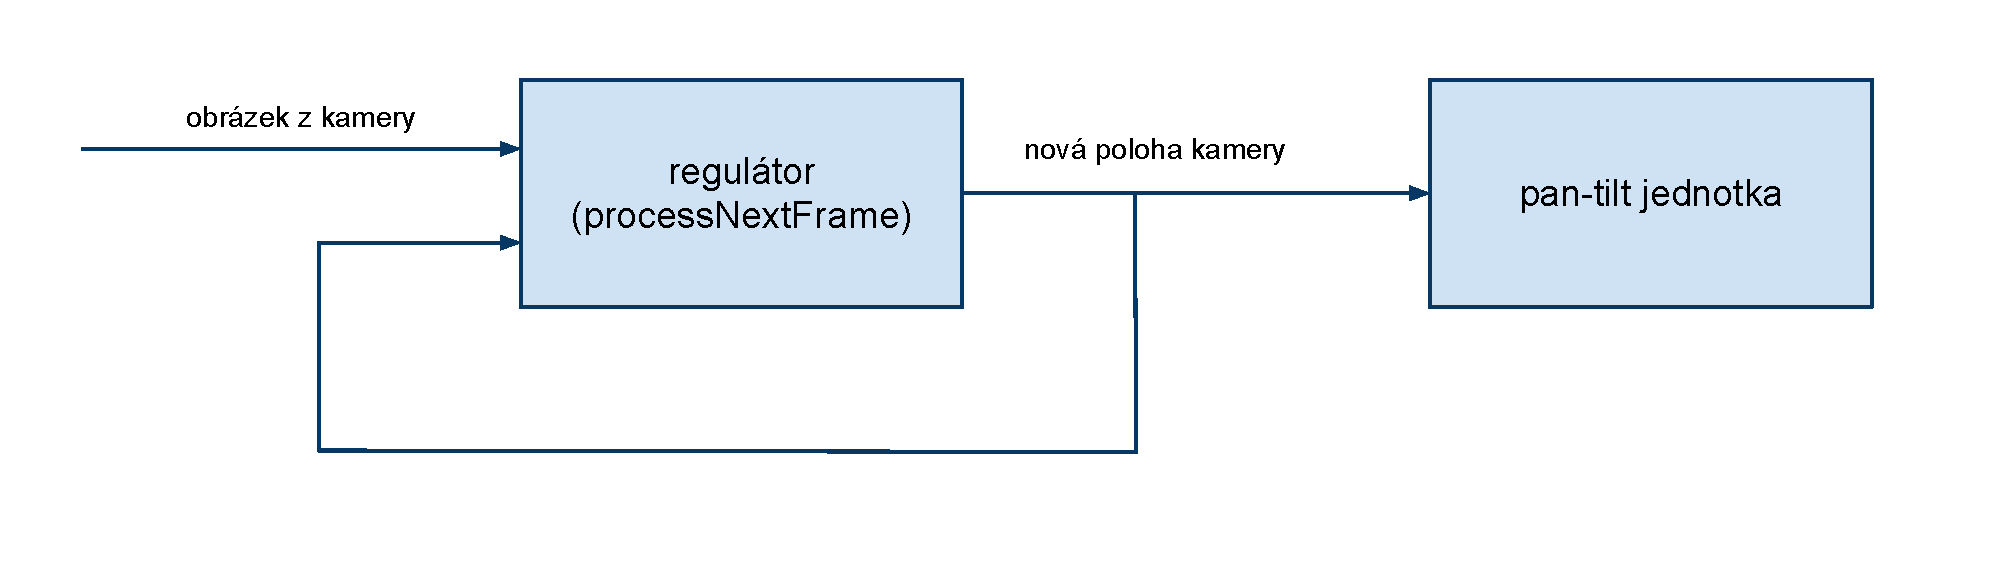
\includegraphics[width=1\columnwidth]{pics/schema_ridiciho_systemu}
     \caption{Schéma řídícího systému\label{fig:rid_system}}
\end{figure}


\section{Implementace}

\subsection{Hlavní metody}

Program se spouští hlavní metodou \textit{startMosquitoHunter}:

Po spuštění funce se zinicializuje servo mechanismus tak, aby se kamera nastavila na střed obrazovky, jedná se o startovní konfiguraci, ve která kamera čeká dokud komár nepřilétne do jejího zorného pole. Tento postup je sice pasivní, ale experimenty prokázaly, že oproti aktivímu vyhledávání komára na počátku programu je časově efektivnější. Aktivním vyhledáváním je myšlen algoritmus, kdy kamera sekvenčně snímala pruhy obrazovky a vyhledávala komára.

Jako další krok se zincializuje kamera a s periodou $X? s$ se s využitím callback funkce volá \textit{processNextFrame}, která zahrnuje hlavní chod programu. Perioda je nastavena jako základní testovací, její hodnota se bude ladit do třetí etapy tak, aby byla optimální a omezená pouze parametry kamery a mechanické soustavy. 

\begin{figure}[!h]
    \centering
     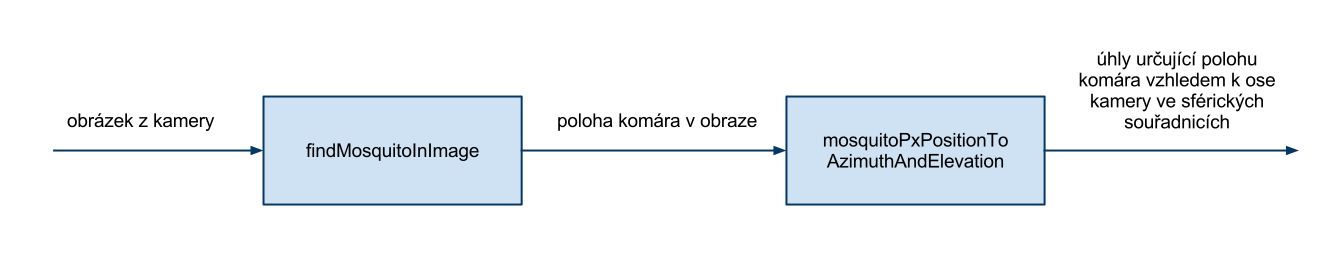
\includegraphics[width=1\columnwidth]{pics/zpracovani_obrazu_z_kamery}
     \caption{Zpracování obrazu z kamery\label{fig:rid_system}}
\end{figure}


\vspace{0.5cm}
\textit{processNextFrame}

Tato funkce pracuje s jedním obrazem získaným z kamery, upraví ho využitím deBayrizace. Takto upravený obraz předá funkci \textit{findMosquitoInImage}, jejíž návratové hodnoty jsou $x, y$ souřadnice středu komára v obraze. Tyto hodnoty jsou předány funkci \textit{mosquitoPxPositionToAzimuthAndElevation}, která vypočte hodnoty azimutu a elevace. V těle funkce \textit{processNextFrame} je implementován PI regulátor. Pozice kamery je saturována na hodnoty, ve kterých je očekáván komár, tedy na hodnoty odpovídající kraji monitoru. 

\vspace{0.5cm}
\textit{findMosquitoInImage}

K získání polohy komára v obrazu z kamery byl použit jednoduchý algoritmus využívající morfologických funkci Matlabovského Image Processing Toolboxu. Jedná se o funkce \textit{bwlabel} pro nalezení souvislých oblastí a funkce \textit{regionprops} pro určení délky (vlastnost \textit{MajorAxisLength}) a plochy (vlastnost \textit{Area}) těchto oblastí.

%kdyz je to efektivnejsi, proc to nedelame? '' empiricky urcena hodnota? histogram se nelibil? '' jejíchž?
Komár zobrazovaný na monitoru pracoviště je představován černým čtvercem na bílém pozadí. Barevná informace je proto zanedbávána a použit je pouze obrázek ve stupních šedi (efektivnější by bylo použít pouze jednu z barevných složek). Tento obrázek je následně oprahován, přičemž jako mez je použita empiricky určená hodnota. V oprahovaném binárním obrázku jsou nalezeny souvislé oblasti právě využitím funkce \textit{bwlabel}. Z nalezených oblastí je vybrána ta, kterou považujeme za komára. Pro toto rozhodnutí jsou použity vlastnosti \textit{MajorAxisLenght} a \textit{Area} oblastí. Jsou vyloučeny takové oblasti, jejíchž plocha je větší než $3000$ pixelů nebo jejich délka je více než $50$ pixelů. Tyto hodnoty byly nastaveny na základě maximálních parametrů komára a dostatečné rezervy. Ze zbývajících oblastí je vybrána ta, která má největší plochu. Pro tuto oblast je určena poloha středu v pixelových souřadnicích a tato infromace je návratová hodnota funkce \textit{findMosquitoInImage}.

%Z barevného obrázku se nejprve vytvoří obrázek šedotónový uložený ve formátu uint8. Po té se naleznou oblasti, ve kterých je podezření na komára na základě znalosti, že komár je tmavý obrazec na světlém pozadí. Tyto oblasti se vyhodnocují na základě histogramu obrázku, hodnoty světlejší než intenzita 200 se zahodí. Tato hodnota byla experimentálně určena, s dostatečnou jistotou oblast komára není světlejší, maximální světlost byla pozorována pod hodnotou 100. Ve zbylé části histogramu se vyhodnotí maximum četností. Práh pro detekci komára je stanoven jako dvojnásobek této hodnoty – dostatečné pokrytí rozložení intenzit kolem maxima. 

\vspace{0.5cm}
\textit{mosquitoPxPositionToAzimuthAndElevation}

V této funkci se přepočtou souřadnice v pixelech obrazu na informaci o azimutu a elevaci.

%konkrétnější popis

\subsection{Pomocné metody}

\textit{addCrosshairToThePicture}

Vstup:
Do středu obrázku vykreslí kříž zadané tloušťky. 


\section{Experimentální výsledky}

%Výpočetní rychlost algoritmu byla optimalizována, při měření času funkcemi tic, toc byl v průměru naměřen čas 0,08 s.

%?zkontrolovat hodnotu
\section{Diskuze}
\section{Závěr}







\end{document}
